% fs-01-OrganizationData.tex

\documentclass[xcolor=dvipsnames]{beamer}

\usepackage{graphicx}
\usepackage{wrapfig}
\usepackage{colortbl}
\usepackage{alltt}
\definecolor{myblue}{rgb}{0.8,0.85,1}

\mode<presentation>
{
  \usetheme{Warsaw}
  \setbeamercovered{transparent}
}
% \usecolortheme[named=OliveGreen]{structure}
\setbeamertemplate{navigation symbols}{} 
\setbeamertemplate{blocks}[rounded][shadow=true] 

\newif\ifBCITCourse
\BCITCoursetrue
% \BCITCoursefalse
\newif\ifWhichCourse
\WhichCoursetrue
% \WhichCoursefalse
\ifBCITCourse
\ifWhichCourse
\newcommand{\CourseName}{Statistics for Food Technology}
\newcommand{\CourseNumber}{MATH 2441}
\newcommand{\CourseInst}{BCIT}
\else
\newcommand{\CourseName}{Calculus for Geomatics}
\newcommand{\CourseNumber}{MATH 2511}
\newcommand{\CourseInst}{BCIT}
\fi
\else
\newcommand{\CourseName}{Philosophy and Literature}
\newcommand{\CourseNumber}{PHIL 375}
\newcommand{\CourseInst}{UBC}
\fi

\title{Organization of Data}
\subtitle{{\CourseNumber}, BCIT}

\author{\CourseName}

\date{January 4, 2018}

% \begin{figure}[h]
% 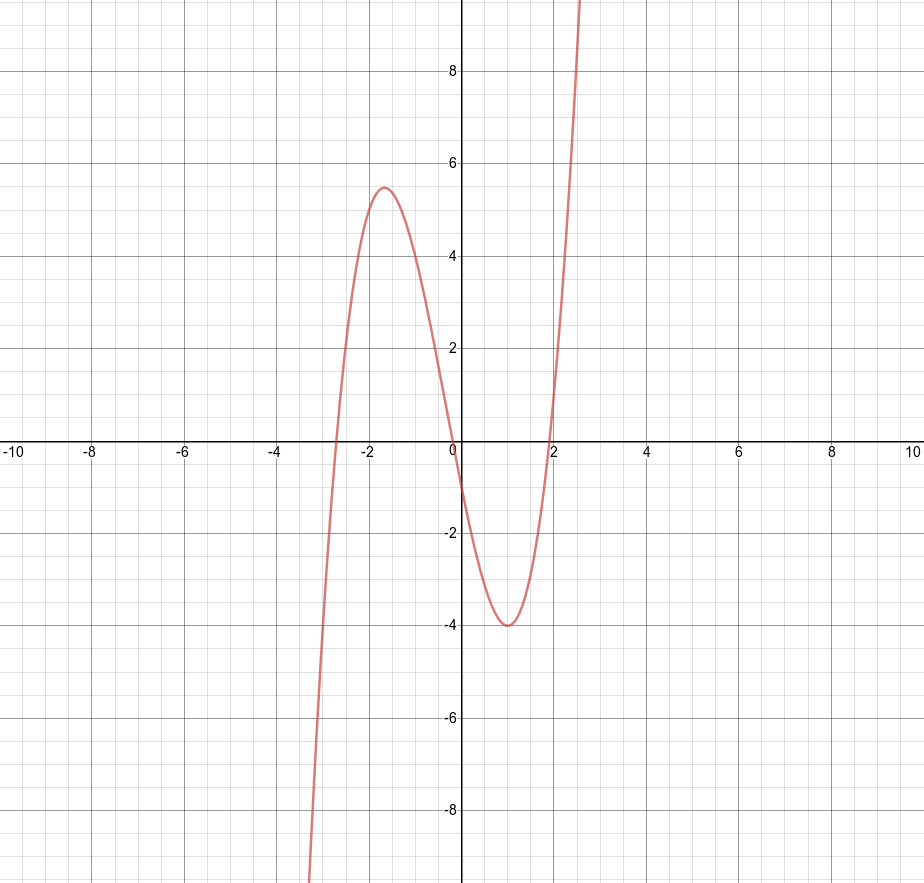
\includegraphics[scale=.3]{./extrema1.png}
% \end{figure}

% Command             10pt    11pt    12pt
% \tiny               5       6       6
% \scriptsize         7       8       8
% \footnotesize       8       9       10
% \small              9       10      10.95
% \normalsize         10      10.95   12

\begin{document}

\begin{frame}
  \titlepage
\end{frame}

\begin{frame}
  \frametitle{Introductory Concepts in Statistics I}
  \begin{itemize}
  \item<1-> A \alert{population} is the complete collection of all
    measurements or data that are being considered.
  \item<2-> A \alert{census} is the collection of data from every
    member of the population.
  \item<3-> A \alert{sample} is a subcollection of members selected
    from a population.
  \end{itemize}
\end{frame}

\begin{frame}
  \frametitle{Introductory Concepts in Statistics II}
  \begin{itemize}
  \item<1-> A \alert{voluntary response sample} or
    \alert{self-selected sample} is one in which the respondents
    themselves decide whether to be included.
  \item<2-> A \alert{random sample} is one in which each member has
    the same probability of being selected.
  \item<3-> A \alert{stratified random sample} is one in which random
    samples from subgroups are drawn and proportionally combined to
    form the complete sample.
  \end{itemize}
\end{frame}

\begin{frame}
  \frametitle{Introductory Concepts in Statistics III}
  \begin{itemize}
  \item<1-> A \alert{parameter} is a numerical measurement describing
    some characteristic of the population.
  \item<2-> A \alert{statistic} is a numerical measurement describing
    some characteristic of a sample.
  \end{itemize}
\end{frame}

\begin{frame}
  \frametitle{Introductory Concepts in Statistics IV}
  \begin{itemize}
  \item<1-> \alert{Quantitative} (or \alert{numerical}) data consist
    of numbers representing counts or measurements.
  \item<2-> \alert{Categorical} (or \alert{qualitative}) data consist
    of names or labels that are not numbers representing counts or
    measurements.
  \end{itemize}
\end{frame}

\begin{frame}
  \frametitle{Introductory Concepts in Statistics V}
  \begin{itemize}
  \item<1-> \alert{Discrete} data result when the data values are
    quantitative and the number of values is finite or countable.
  \item<2-> \alert{Continuous} data result when the data values are
    quantitative and the number of values is infinite and not
    countable.
  \end{itemize}
Here is an example for infinite discrete outcomes (this is rare). Roll
a die until you roll a six. There are infinitely many ways to do this,
but the data is not continuous.
\end{frame}

\begin{frame}
  \frametitle{Introductory Concepts in Statistics VI}
  \begin{itemize}
  \item<1-> \alert{Blinding} is when the subject doesn't know whether
    they are receiving a treatment or a placebo.
  \item<2-> The \alert{placebo effect} occurs when an untreated
    subject reports an improvement in symptoms because of their
    participation in the study.
  \item<3-> An experiment is \alert{double-blind} when it is blind and
    the experimenter also doesn't know whether they are applying a
    treatment or a placebo.
  \end{itemize}
\end{frame}

\begin{frame}
  \frametitle{Correlation Does Not Imply Causation}
\alert{Confounding} occurs in an experiment when the investigators are
not abloe to distinguish among the effects of different factors.
\begin{figure}[h]
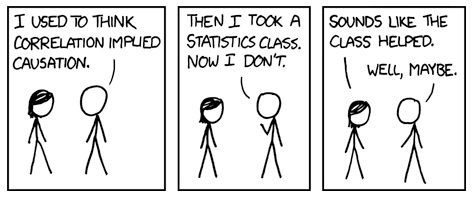
\includegraphics[scale=.3]{./xkcd-causation-correlation.png}
\end{figure}
Examples: 
\begin{enumerate}
\item<1-> astrological sign and IQ in elementary school
\item<2-> soft drinks and obesity
\item<3-> birth control pills and thrombosis
\end{enumerate}
\end{frame}

\begin{frame}
  \frametitle{Modes of Data Presentation}
The three modes of data presentation.
\begin{itemize}
\item textual
\item tabular
\item graphical
\end{itemize}
\end{frame}

\begin{frame}
  \frametitle{Textual}
Example for textual data presentation.
\begin{block}{Philippine Stock Market}
The Philippine Stock Exchange composite index lost 7.19 points to
2,099.12 after trading between 2,095.30 and 2,108.47. Volume was 1.29
billion shares worth 903.15 million pesos (16.7 million dollars). The
broader all share index gained 5.21 points to 1,221.34. (From: Freeman
dated March 17, 2005)
\end{block}
\end{frame}

\begin{frame}
  \frametitle{Types of Graphs}
Four types of graphs.
\begin{itemize}
\item Line plot
\item Pie chart
\item Bar plot
\item Multi-bar graph
\item Histogram
\end{itemize}
\end{frame}

\begin{frame}
  \frametitle{Line Plot}
Usually suitable for data on a timeline. Here is an example. Rainy
days in Vancouver.

\begin{tabular}{|l|r|r|r|r|}\hline
  & Q1 & Q2 & Q3 & Q4 \\ \hline
2012 & 55 & 43 & 13 & 65 \\ \hline
2013 & 53 & 41 & 27 & 35 \\ \hline
2014 & 45 & 38 & 18 & 54 \\ \hline
2015 & 49 & 19 & 25 & 53 \\ \hline
2016 & 61 & 28 & 27 & 69 \\ \hline
\end{tabular}
\end{frame}

\begin{frame}
  \frametitle{Data for Line Plot Example}
Here is the file \texttt{fs01.csv}. On a Windows computer, open the
program called Notepad and paste the data into it. Then save as
\texttt{fs01.csv}. You can then open this file in R Studio, for
example (but also in other statistical software, such as minitab or
excel). 
\begin{alltt}
\tiny
year,quarter,dor\newline
2012,Q1,55\newline
2012,Q2,43\newline
2012,Q3,13\newline
2012,Q4,65\newline
2013,Q1,53\newline
2013,Q2,41\newline
2013,Q3,27\newline
2013,Q4,35\newline
2014,Q1,45\newline
2014,Q2,38\newline
2014,Q3,18\newline
2014,Q4,54\newline
2015,Q1,49\newline
2015,Q2,19\newline
2015,Q3,25\newline
2015,Q4,53\newline
2016,Q1,61\newline
2016,Q2,28\newline
2016,Q3,27\newline
2016,Q4,69
\end{alltt}
\end{frame}

% \begin{frame}
%   \frametitle{Line Plot Example By Quarter}
% In R Statistics, use the file \texttt{fs01.csv} and the following
% code.
% \begin{alltt}
% \small
% a<-read.table("fs01.csv",sep=",",header=TRUE)\newline
% b1<-subset(a,quarter=="Q1",select=c(dor))\newline
% b2<-subset(a,quarter=="Q2",select=c(dor))\newline
% b3<-subset(a,quarter=="Q3",select=c(dor))\newline
% b4<-subset(a,quarter=="Q4",select=c(dor))\newline
% ylima<-min(a[[3]])-3\newline
% ylimb<-max(a[[3]])+3\newline
% plot(b1[[1]],type="o",ylim=c(ylima,ylimb),col="blue")\newline
% lines(b2[[1]],type="o",col="red")\newline
% lines(b3[[1]],type="o",col="green")\newline
% lines(b4[[1]],type="o",col="yellow")
% \end{alltt}
% \end{frame}

% \begin{frame}
%   \frametitle{Line Plot Example By Quarter}
% \begin{figure}[h]
% 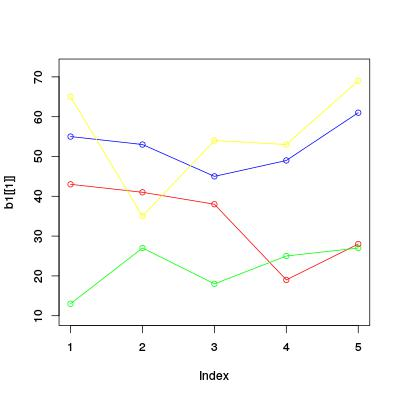
\includegraphics[scale=.6]{./lineplot1.jpg}
% \end{figure}
% \end{frame}

\begin{frame}
  \frametitle{Line Plot Example By Year}
In R Statistics, use the file \texttt{fs01.csv} and the following
code.
\begin{alltt}
\small
a<-read.table("fs01.csv",sep=",",header=TRUE)\newline
c1<-subset(a,year=="2012",select=c(dor))\newline
c2<-subset(a,year=="2013",select=c(dor))\newline
c3<-subset(a,year=="2014",select=c(dor))\newline
c4<-subset(a,year=="2015",select=c(dor))\newline
c5<-subset(a,year=="2016",select=c(dor))\newline
ylima<-min(a[[3]])-3\newline
ylimb<-max(a[[3]])+3\newline
plot(c1[[1]],type="o",ylim=c(ylima,ylimb),col="blue")\newline
lines(c2[[1]],type="o",ylim=c(ylima,ylimb),col="red")\newline
lines(c3[[1]],type="o",ylim=c(ylima,ylimb),col="green")\newline
lines(c4[[1]],type="o",ylim=c(ylima,ylimb),col="yellow")\newline
lines(c5[[1]],type="o",ylim=c(ylima,ylimb),col="orange")
\end{alltt}
\end{frame}

\begin{frame}
  \frametitle{Line Plot Example By Year}
\begin{figure}[h]
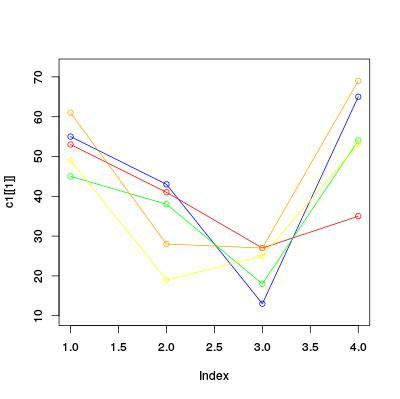
\includegraphics[scale=.6]{./lineplot2.jpg}
\end{figure}
\end{frame}

\begin{frame}
  \frametitle{Pie Chart}
Pie charts are often used for tabular representations of categorical
data. Consider the following data set \texttt{fs02.csv} and the
corresponding chart on the next slide.
\begin{alltt}
\small
party,votes\newline
LIB,6943276\newline
CON,5613614\newline
NDP,3470350\newline
BQU,821144\newline
GRN,602944
\end{alltt}
\end{frame}

\begin{frame}
  \frametitle{Pie Chart Graph}
We are using the following R commands: 
\begin{alltt}
\small
d<-read.table("fs02.csv",sep=",",header=TRUE)\newline
pie(d[[2]],label=d[[1]])
\end{alltt}

However, pie charts are not recommended for visualizing statistical
data. Bar plots make differences between data points more clear.
\begin{figure}[h]
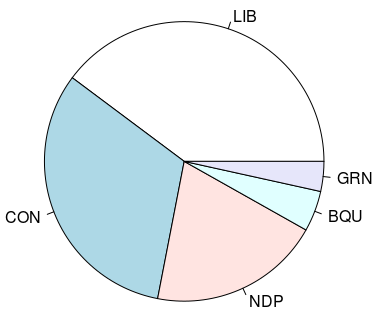
\includegraphics[scale=.5]{./pie.png}
\end{figure}
\end{frame}

\begin{frame}
  \frametitle{Bar Plot Graph}
\begin{figure}[h]
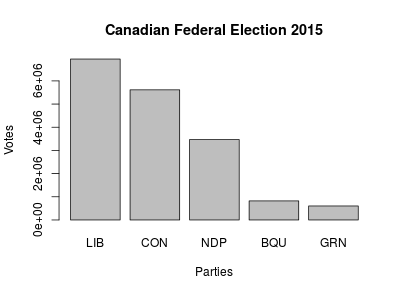
\includegraphics[scale=.5]{./barplot.png}
\end{figure}
We have used the following R command: 
\begin{alltt}
\small
barplot(d[[2]], main="Canadian Federal Election 2015",\newline
xlab="Parties",ylab="Votes",names.arg=d[[1]])
\end{alltt}
\end{frame}

\begin{frame}
  \frametitle{Multi-Bar Graph}
Use the following R commands for a multi-bar graph of tabular data: 
\begin{alltt}
\small
e<-read.table("fs03.csv",sep=",",header=TRUE)\newline
barplot(as.matrix(e),beside=TRUE,col=rainbow(4))
\end{alltt}
Here is how to organize the data in the file \texttt{fs03.csv} for these commands:
\begin{alltt}
\small
y2012,y2013,y2014,y2015,y2016\newline
55,53,45,49,61\newline
43,41,38,19,28\newline
13,27,18,25,27\newline
65,35,54,53,69
\end{alltt}
These are the rainy days in Vancouver as in \texttt{fs01.csv}, but
organized in tabular form.
\end{frame}

\begin{frame}
  \frametitle{Multi-Bar Graph}
\begin{figure}[h]
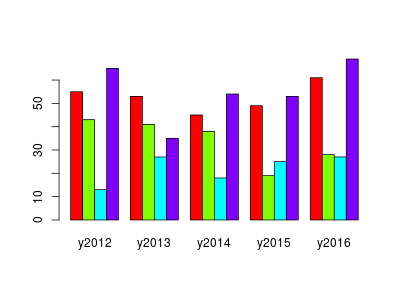
\includegraphics[scale=.8]{./mbg.png}
\end{figure}
\end{frame}

\begin{frame}
  \frametitle{Histogram}
We use histograms for continuous data, bar plots for discrete data.
Use the R command
\begin{alltt}
  x<-round(rnorm(200,71,11)*100)/100
\end{alltt}
for the grades of 200 students in a course. Then use
\begin{alltt}
  hist(x)
\end{alltt}
for the histogram. There are different suggestions for what the ideal
length of intervals is for a histogram. $\sqrt{n}$ is one useful rule
of thumb, where $n$ is the sample size (number of data points in the
data set). 
\end{frame}

\begin{frame}
  \frametitle{Histogram}
\begin{figure}[h]
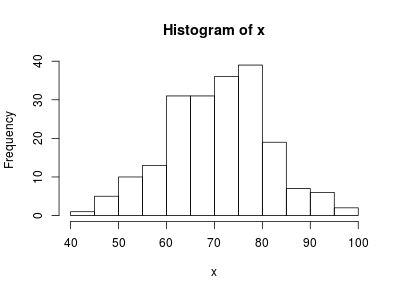
\includegraphics[scale=.8]{./histogram.png}
\end{figure}
\end{frame}

\begin{frame}
  \frametitle{Characterizing Data Sets}
  The following serve to characterize data sets without listing the
  data:
  \begin{itemize}
  \item measures of centre
  \item measures of dispersion
  \item measures of position
  \end{itemize}
\end{frame}

\begin{frame}
  \frametitle{Measures of Centre: Mean}
  \begin{equation}
    \label{eq:daechuev}
    \mbox{mean}=\frac{\sum{}x}{n}
  \end{equation}
  where $n$ is the number of data points in your quantitative data set
  and $x$ is your data set. Mathematically speaking, $x$ is an
  $n$-dimensional vector $x=(x_{1},{\ldots},x_{n})$ and $\sum{}x$
  means
  \begin{equation}
    \label{eq:aethecux}
    \sum{}x=x_{1}+{\ldots}x_{n}
  \end{equation}
Often, we write $\mu$ for the mean of a
  population and $\bar{x}$ for the mean of a sample.
\end{frame}

\begin{frame}
  \frametitle{Frequency Distributions}
Often, data is provided in the form of a frequency distribution. For
example, when I asked a class of statistics students about the number
of countries they had visited in their lifetime, the response was as
follows (given as an R command),
\begin{alltt}
\small
cn<-c(5,4,7,3,6,4,3,4,2,4,4,2,4,3,2,4,4)
\end{alltt}
A more intelligible way to display the data is to provide a frequency
distribution.
\begin{alltt}
> table(cn)\newline
cn\newline
2 3 4 5 6 7 \newline
3 3 8 1 1 1
\end{alltt}
There are 3 people who have been to 2 countries, 3 people who have
been to 3 countries, 8 people who have been to 4 countries, 1 person
who has been to 5 countries, and so on.
\end{frame}

\begin{frame}
  \frametitle{Calculating the Mean from a Frequency Distribution}
If you have a frequency distribution (usually of a sample, so we will
call the mean $\bar{x}$), the mean is 
\begin{equation}
  \label{eq:eogheivi}
  \bar{x}=\frac{\sum{}\left(f\cdot{}x\right)}{\sum{}f}
\end{equation}
For the example in the last slide,
\begin{equation}
  \label{eq:uevuemoo}
  \bar{x}=\frac{2\cdot{}3+3\cdot{}3+4\cdot{}8+5\cdot{}1+6\cdot{}1+7\cdot{}1}{3+3+8+1+1+1}\approx{}3.82
\end{equation}
In R, you can also simply use the command \texttt{mean}. Notice that
\texttt{mean(x)} and \texttt{sum(x)/length(x)} will give you the same
number.
\end{frame}

\begin{frame}
  \frametitle{Exercises}
  {\ubung} Find the mean of the following five counts for Chips Ahoy
  chocolate chip cookies: 22 chips, 22, chips, 26 chips, 24 chips, and
  23 chips.

  \bigskip

  {ubung} Anne measures the temperature in her walk-in freezer. She
  measures $-23^{\circ}$C once; $-22^{\circ}$C 31 times;
  $-21^{\circ}$C 13 times; $-0^{\circ}$C 7 times; $-18^{\circ}$C
  twice. What is the mean temperature given this dataset?
\end{frame}

\begin{frame}
  \frametitle{Measures of Centre: Median}
The median is the value in the middle. If there is an even number of
data points, the median is the mean of the two data points in the
middle. To find the median, sort the data points. For example, the
numbers of countries visited are

\medskip

\begin{tabular}{|c|c|c|c|c|c|c|c|c|c|c|c|c|c|c|c|c|}\hline
2&2&2&3&3&3&4&4&\alert{4}&4&4&4&4&4&5&6&7 \\ \hline
\end{tabular}

\medskip

The value in the middle is the number 4, which is also the median of
the data. It is quite similar to the mean, which is approximately 3.82.
\end{frame}

\begin{frame}
  \frametitle{Difference Between Mean and Median}
Imagine we had one more student in the class who was a world traveler.
She had visited 112 countries! The mean is now
\begin{equation}
  \label{eq:zephahwu}
  \bar{x}=\frac{\sum{}x}{n}=\frac{177}{18}\approx{}9.83
\end{equation}
A mean of 9.83 is no longer a good summary of the data. Let's see if
the median does better.

\medskip

\begin{tabular}{|c|c|c|c|c|c|c|c|c|c|c|c|}\hline
2&2&{\ldots}&4&4&\alert{4}&\alert{4}&4&{\ldots}&6&7&112 \\ \hline
\end{tabular}

\medskip

The new median is $(4+4)/2=4$, which is a much better summary of the
data, pretty much ignoring the outlier.
\end{frame}

\begin{frame}
  \frametitle{Measures of Centre: Mode}
The \alert{mode} of a data set is the value that occurs with the
greatest frequency. In the numbers of countries visited example the
mode is clearly 4. To be precise, the mode of a data set is itself a
set of numbers. A data set can have one mode, as in our example, but
if more values are repeated the same number and a maximum number of
times, they are all modes. If no data point is repeated, the data set
has no mode.
\end{frame}

\begin{frame}
  \frametitle{Measures of Centre: Midrange}
The \alert{midrange} is the midpoint between the maximum and the
minimum data points. It is very sensitive to outliers! For example,
\begin{equation}
  \label{eq:nahjuise}
  \mbox{midrange}=\frac{7+2}{2}=4.5
\end{equation}
without the outlier, and
\begin{equation}
  \label{eq:foofieng}
  \mbox{midrange}=\frac{112+2}{2}=57
\end{equation}
with the outlier in the numbers of countries visited example.
\end{frame}

\begin{frame}
  \frametitle{Measures of Dispersion: Motivation}
Have a look at these two different data sets.
\begin{alltt}
x1<-c(12,12,12,12,12,12,11,12,12,13,12,12,12,12)
\end{alltt}
and
\begin{alltt}
x2<-c(15,10,14,7,17,15,11,18,12,12,15,9,7,6)
\end{alltt}
The mean of both data sets is 12. The median of both data sets is 12.
However, something about these two data sets is different. \texttt{x2}
is more dispersed than \texttt{x1}, which means that the data is
spread out more. There is more variation in \texttt{x2}. We try to
capture this variation by finding measures of dispersion.
\end{frame}

\begin{frame}
  \frametitle{Measures of Dispersion: Range}
One very simple measure of dispersion is the \alert{range}, which is
just the lowest value subtracted from the highest value. 
\begin{equation}
  \label{eq:ungoliex}
  \mbox{range of \texttt{x1} }=13-11=2
\end{equation}
\begin{equation}
  \label{eq:aengoore}
  \mbox{range of \texttt{x2} }=18-6=12
\end{equation}
The problem is outliers: they would change the range significantly
while many other data points would be ignored. Another possibility is
to count up the difference between data points and the mean. Can you
guess what the problem of this measure would be?
\end{frame}

\begin{frame}
  \frametitle{Measures of Dispersion: Midquartile}
The \alert{interquartile range} is a measure of dispersion which is not as
vulnerable to outliers as the range. The interquartile range is
visually best represented in a box-and-whiskers display. For the 200
students, the box-and-whiskers display is generated by the following R
Studio command,
\begin{alltt}
boxplot(x,range=0)
\end{alltt}
\texttt{range=0} means that the plot will not pay attention to
outliers. The default is \texttt{range=1.5}, which will show some
outliers. We will find out how to calculate quartiles in a moment when
we will talk about measures of position.
\end{frame}

% \begin{frame}
%   \frametitle{Box-and-Whiskers Display Without Outliers}
% \begin{figure}[h]
% \includegraphics[scale=.6]{./box.png}
% \end{figure}
% \end{frame}

\begin{frame}
  \frametitle{Box-and-Whiskers Display with Outliers}
\begin{figure}[h]
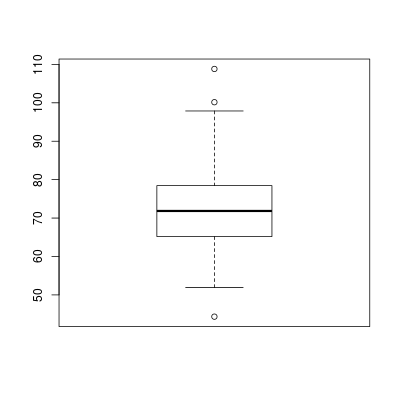
\includegraphics[scale=.6]{./box1.png}
\end{figure}
\end{frame}

\begin{frame}
  \frametitle{Measures of Dispersion: Absolute Value of Deviation}
The difference between data points and the mean always sums to zero!
That is not helpful. If we want to make this measure of dispersion
more useful, we need to sum the \alert{absolute value of deviation}
\begin{equation}
  \label{eq:riquithu}
  \mbox{mean absolute deviation }=\frac{\sum{}\vert{}x-\bar{x}\vert}{n}
\end{equation}
For our examples \texttt{x1} and \texttt{x2}, the mean absolute
deviations are 2 and 44, respectively. Although at first glance this
measure of dispersion looks useful, it makes for very complicated
calculations that can be simplified by choosing a different way to
make all the distances between data points and mean positive: not the
absolute value, but the square of the distance.
\end{frame}

\begin{frame}
  \frametitle{Measures of Dispersion: Variance}
The \alert{variance} is calculated as follows,
\begin{equation}
  \label{eq:roongeef}
   \mbox{variance of a population }=\sigma^{2}=\frac{\sum{}(x-\mu)^{2}}{n}
\end{equation}
Something odd happens when we take the variance of a sample. If we
were to use equation (\ref{eq:roongeef}) to calculate the sample
variance for all possible samples of a population, the mean of these
sample variance would not equal the population variance. This means
that in this case the sample variance would be a \alert{biased
  estimator} of the population variance. We don't want that! To
correct for this problem and define a sample variance which is an
\alert{unbiased estimator} of the population variance, we introduce
\alert{Bessel's correction} and define
\begin{equation}
  \label{eq:ilosoama}
   \mbox{variance of a sample }=s^{2}=\frac{\sum{}(x-\bar{x})^{2}}{n-1}
\end{equation}
\end{frame}

\begin{frame}
  \frametitle{Measures of Dispersion: Standard Deviation}
One disadvantage of the variance is that it is not an intuitive
measurement of dispersion. If we take the square root of the variance,
then we get something similar to the absolute value of deviation,
which tells us approximately how far on average the data points are
from the mean. We call this measurement the \alert{standard
  deviation}
\begin{equation}
  \label{eq:boolaesh}
   \mbox{standard deviation of a population }=\sigma=\sqrt{\frac{\sum{}(x-\mu)^{2}}{n}}
\end{equation}
\begin{equation}
  \label{eq:xeiroong}
   \mbox{standard deviation of a sample }=s=\sqrt{\frac{\sum{}(x-\bar{x})^{2}}{n-1}}
\end{equation}
Why we still sometimes prefer the variance will become
clear on the next slide. The standard deviation, whether with or
without Bessel's Correction, is a biased estimator!
\end{frame}

\begin{frame}
  \frametitle{Bessel's Correction}
\begin{figure}[h]
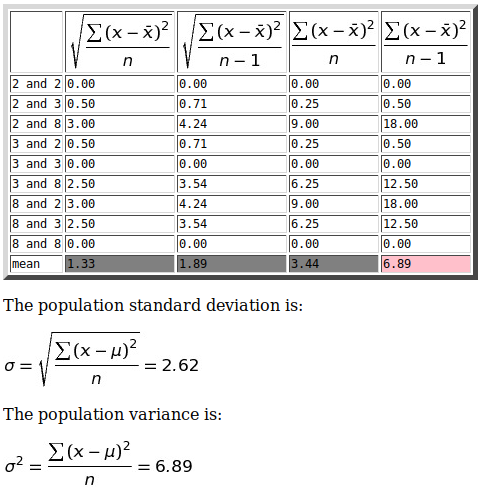
\includegraphics[scale=.45]{./bessel.png}
\end{figure}
\end{frame}

\begin{frame}
  \frametitle{Calculating the Variance I}
It is easiest to calculate the variance using statistical software. In
R Studio, for example,
\begin{alltt}
> var(x1)\newline
[1] 0.1538462\newline
> var(x2)\newline
[1] 14.76923
\end{alltt}
and
\begin{alltt}
> sd(x1)\newline
[1] 0.3922323\newline
> sd(x2)\newline
[1] 3.843076
\end{alltt}
\end{frame}

\begin{frame}
  \frametitle{Calculating the Variance II}
When you do have to calculate the variance by hand, it is helpful to
use the following shortcut formula,
\begin{equation}
  \label{eq:eecheaxe}
s^{2}=\frac{\sum(x-\bar{x})^{2}}{n-1}=\frac{\sum{}x^{2}-\frac{\left(\sum{}x\right)^{2}}{n}}{n-1}
\end{equation}
because you do not have to keep entering the mean, which may contain
numerous significant digits.
\end{frame}

\begin{frame}
  \frametitle{Variance for a Frequency Distribution I}
Consider the data set \texttt{x3}
\begin{alltt}
4,4,2,2,4,3,3,3,1,4,4,1,2,2,2,4,2,1,2,1,1,2,3,3,2,3,3,3
\end{alltt}
We can summarize the data in a frequency distribution
\begin{alltt}
> table(x3)\newline
x3\newline
1 2 3 4 \newline
5 9 8 6 
\end{alltt}
\end{frame}

\begin{frame}
  \frametitle{Variance for a Frequency Distribution II}
Remember that in equation (\ref{eq:eogheivi}) we calculated the mean using a
formula for the frequency distribution,
\begin{equation}
  \label{eq:beingeip}
  \bar{x}=\frac{\sum{}\left(f\cdot{}x\right)}{\sum{}f}
\end{equation}
We can do the same for the variance and the standard deviation,
\begin{equation}
  \label{eq:iefoopoo}
  s^{2}=\frac{\sum{}\left(f\cdot{}x^{2}\right)-\frac{\left(\sum{}f\cdot{}x\right)^{2}}{\sum{}f}}{\sum{}f-1}
\end{equation}
Remember that $n=\sum{}f$.
\end{frame}

\begin{frame}
  \frametitle{Measures of Position: Quartiles}
Sometimes we want to know where a data point approximately ranks in
relation to other data points. For a more finely-grained measure of
position, we use percentiles. For a more coarsely-grained measure of
position, we use quartiles. Let's use again the R command
\begin{alltt}
  x<-round(rnorm(200,71,11)*100)/100
\end{alltt}
for the grades of 200 students in a course. On the next slide, you can
see the random numbers generated when I just now ran this command in R Studio.
\end{frame}

\begin{frame}
  \frametitle{Measures of Position: Quartiles}
\begin{alltt}
\footnotesize
  [1]  58.52  74.38  80.79  84.24  86.61  70.92  86.98  76.02  70.67  66.10\newline
 [11]  62.01  63.41  76.33  68.60  73.50  64.15  85.85  86.22  76.80  71.12\newline
 [21]  78.29  52.77  81.25  57.98  66.09  92.43  71.19  65.26  96.96  55.92\newline
 [31]  71.87  70.31  66.84  69.42  67.90  66.46  69.87  72.35  76.83  58.30\newline
 [41]  61.90  57.93  74.90  97.23  87.41  74.86  77.69  63.41  53.55  78.95\newline
 [51]  78.76  71.04  68.63  70.10  77.72  94.69  64.18  76.67  70.97  83.96\newline
 [61]  70.93  75.89  65.19  60.34  64.89  81.38  65.59  72.89  74.22  64.68\newline
 [71]  54.10  84.13  79.10  59.91  74.13  60.49  72.70  68.50  87.30  75.63\newline
 [81]  83.24  71.80  75.54  64.11  77.46  82.05  74.20  72.45  75.03  53.60\newline
 [91]  54.20  65.16  81.77  63.27  57.38  83.93  72.36  63.62  73.02  72.18\newline
[101]  54.66  84.89  58.05  70.27  80.31  76.43  70.66  71.31  86.39  77.85\newline
[111]  73.52  68.07  44.34  62.52  81.15  70.20  76.16  86.35  64.60  85.13\newline
[121]  61.21  65.25  72.94  61.48  90.48  80.50 108.81  57.91  73.53  65.53\newline
[131]  58.08  78.47  75.61  51.90  76.72  70.57  65.18  90.92  86.01  68.36\newline
[141]  78.16  54.97  81.10  75.30  52.39  68.64  82.96  71.82  80.44  59.15\newline
[151] 100.15  54.56  52.91  67.48  75.07  61.07  71.14  58.55  84.35  67.56\newline
[161]  94.91  78.32  70.50  75.73  67.25  71.49  62.55  68.54  59.55  63.01\newline
[171]  65.63  83.72  70.64  82.58  71.13  69.20  77.55  74.76  72.95  61.53\newline
[181]  73.04  84.79  64.35  85.49  78.86  56.27  74.11  97.87  72.58  92.96\newline
[191]  72.99  66.93  78.41  69.93  67.88  80.88  70.84  69.55  74.69  89.32
\end{alltt}
\end{frame}

\begin{frame}
  \frametitle{Measures of Position: Quartiles}
  Let's say you are student number 111, and your score is 73.52\%. The
  students are divided up into four groups of approximately the same
  size. The first quartile $Q_{1}$ is the score which divides the
  first group (with the lowest scores) from the second group. The
  second quartile $Q_{2}$ is the median and divides the second group
  from the third group. The third quartile $Q_{3}$ is the score which divides the
  third group from the fourth group (with the highest scores). 
\end{frame}

\begin{frame}
  \frametitle{Measures of Position: Quartiles}
  To calculate the quartiles you have to rank the data and find the
  corresponding scores, just as you did with the median. Or you use
  statistics software to check out the summary.
\begin{alltt}
> summary(x)\newline
   Min. 1st Qu.  Median    Mean 3rd Qu.    Max. \newline
  44.34   65.19   71.84   72.34   78.42  108.80 
\end{alltt}
\end{frame}

\begin{frame}
  \frametitle{Measures of Position: Quartiles}
  The second quartile is the median. The first quartile separates the
  bottom quarter of the data from the data group that scores higher
  than the bottom quarter and lower than the median. Let $n$ be the
  number of data points. Multiply $n$ by $1/4$ for the first quartile.
  If the result is a whole number $m$, then the first quartile is the
  mean of the two data points in the $m$-th and the $m+1$-th position
  from the bottom. If the result is not a whole number, round up to
  the whole number $m$ and the first quartile is the data point in the
  $m$-th position from the bottom.

  For the third quartile, multiply $n$ by $3/4$.
  If the result is a whole number $m$, then the third quartile is the
  mean of the two data points in the $m$-th and the $m+1$-th position
  from the bottom. If the result is not a whole number, round up to
  the whole number $m$ and the third quartile is the data point in the
  $m$-th position from the bottom.
\end{frame}

\begin{frame}
  \frametitle{Measures of Position: Percentiles}
Percentiles work just like quartiles, using the number 100 instead of
the number 4. Student number 111 turned out to be in the third
group because her score was better than the median but worse than the
third quartile. If we sort the data with the R Studio command
\begin{alltt}
sort(x)
\end{alltt}
we discover that student number 111 is in 115th position (counting
from the bottom), which is the 58th percentile. To find the $k$-th
percentile use
\begin{equation}
  \label{eq:phaecoab}
  \frac{n\cdot{}k}{100}
\end{equation}
For example, the 90th percentile $P_{90}$ is the mean between the 180th and the
181st data point ranked from the bottom (in our case, 85.93\%). As a
reference point, $P_{50}=Q_{2}=$mean.
\end{frame}

\begin{frame}
  \frametitle{Percentiles Flow Chart I}
\begin{figure}[h]
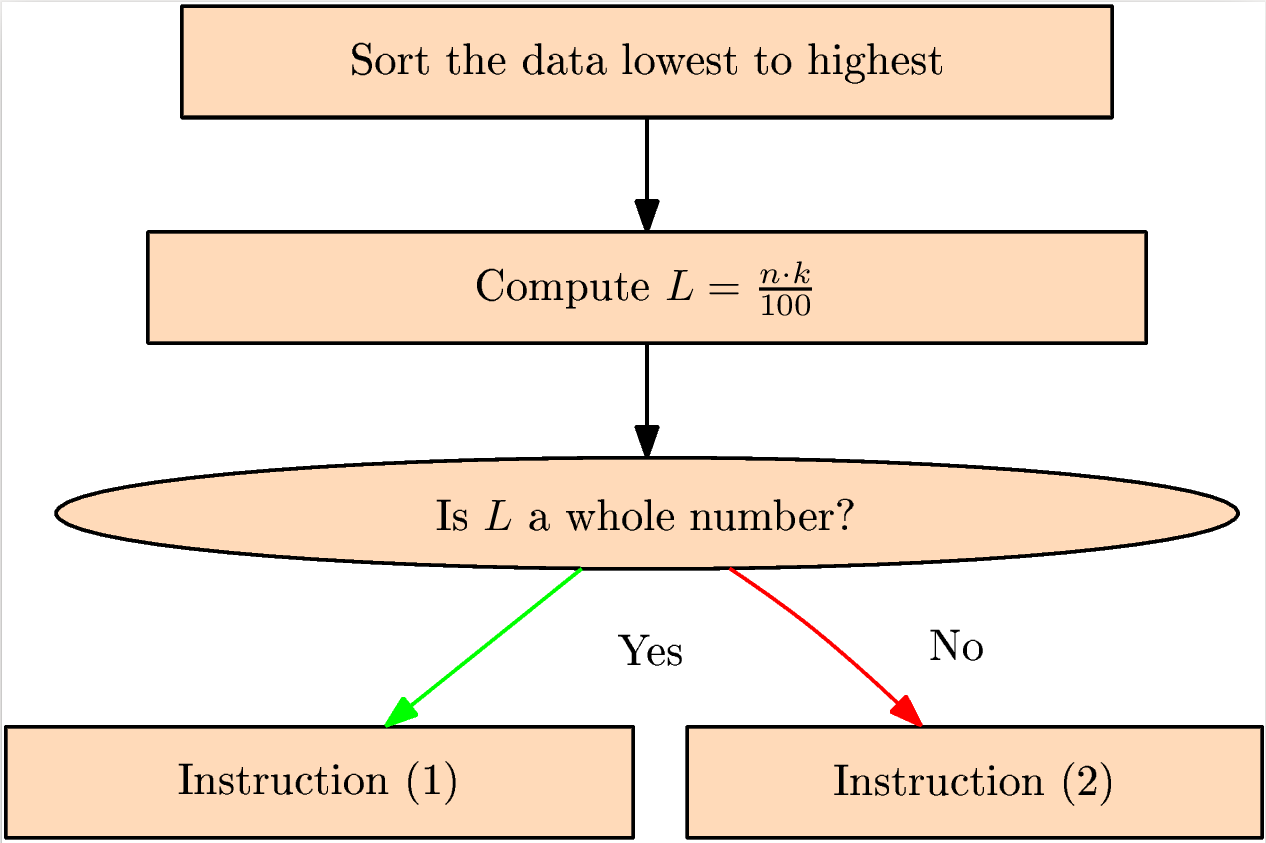
\includegraphics[scale=.15]{./percentile.png}
\end{figure}
Instruction (1): The value of the $k$-th percentile $P_{k}$ is midway
between the $L$-th value and the next value in the sorted set of data.
Find $P_{k}$ by adding the $L$-th value and the next value and
dividing the total by $2$.
\end{frame}

\begin{frame}
  \frametitle{Percentiles Flow Chart II}
\begin{figure}[h]
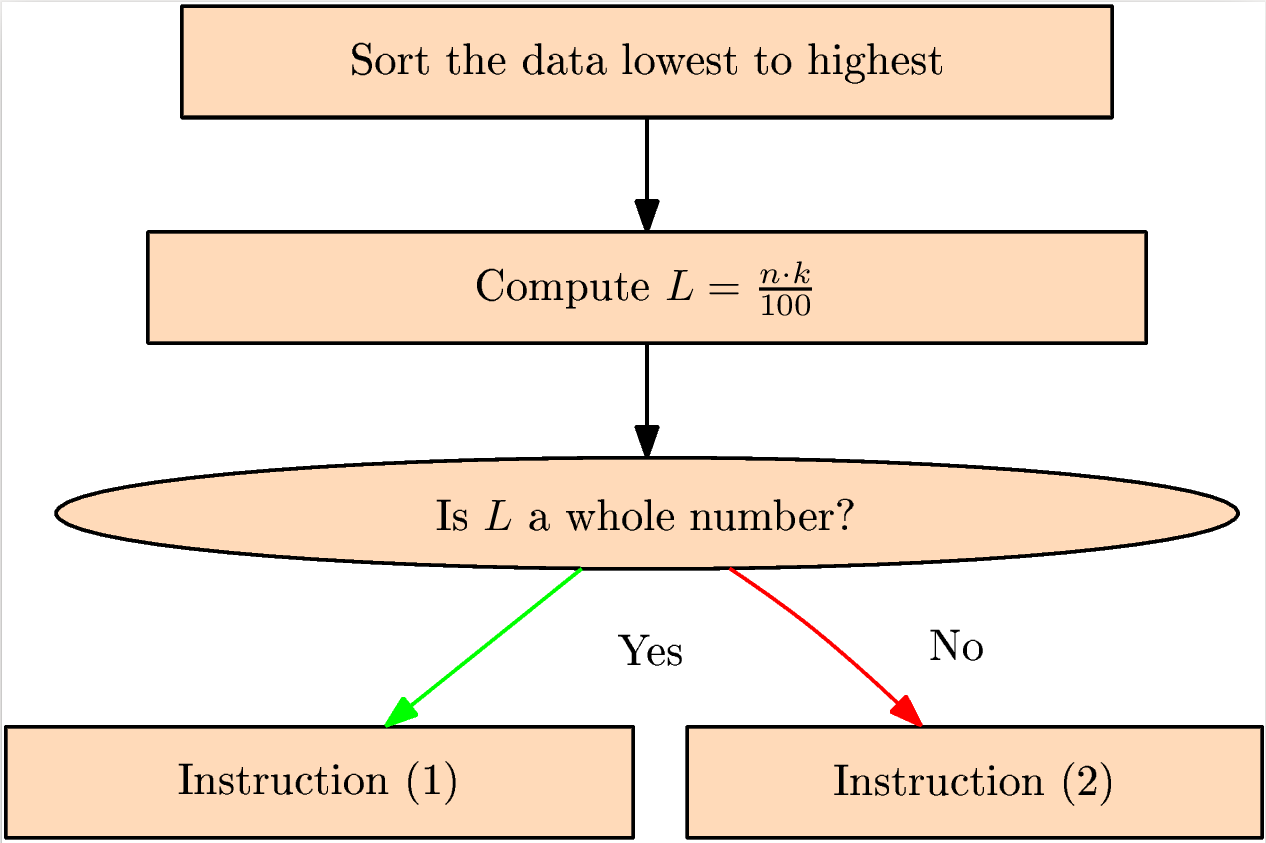
\includegraphics[scale=.15]{./percentile.png}
\end{figure}
Instruction (2): Change $L$ by rounding it up to the next larger
whole number. The value of $P_{k}$ is the $L$-th value, counting
from the lowest.
\end{frame}

\begin{frame}
  \frametitle{End of Lesson}
Next Lesson: Elementary Probability.
\end{frame}

\end{document}
